%---------------------------------------------------------------------------------
\chapter{Fitzhugh-Nagumo Model Example}
\label{chap:fitzhugh-nagumo}
%---------------------------------------------------------------------------------
\section{Background}
\label{sec:background}
We will look into Fitzhugh-Nagumo model as an application of the Python package. The Fitzhugh-Nagumo model describes an excitable system, such as the action potential of cardiac cells. The action potential was first described by Hodgkin and Huxley. Their model were then simplified to the Fitzhugh-Nagumo model, retaining the fast-slow phase and the excitability of the Hodgkin \& Huxley model. \cite{Keener2009}

This model is relevant to my D.Phil.~project as my project will be related to action potential of cardiac muscle cells, an excitable system. I will be working on sodium ion channels of cardiac muscle cells, studying the effect of the flow of sodium ions across the cell membrane on the cell's action potential. Moreover, Fitzhugh-Nagumo model captures all the important features of an action potential, the excitability and the fast-slow phase. Therefore, it is a good simple model to start with.

\section{Fitzhugh-Nagumo model}
\label{sec:FHN}
The definition of Fitzhugh-Nagumo model is
\begin{align}
\label{eqn:FHN}
    \epsilon \frac{dv}{dt} &= f(v) - w + I_{app} \\
    \frac{dw}{dt} &= v - \gamma w \label{eqn:FHN-end}
\end{align}
where $f(v) = v(1-v)(v-\alpha)$, $0 < \alpha < 1$, $\epsilon \ll 1$, $I_{app}$ is the applied current and $t$ is time. The fast $v$ is the excitation variable, while the slow $w$ is the recovery variable.

In this implementation, the parameters are chosen to be $\alpha = 0.1$, $\gamma = 0.5$, $\epsilon = 0.01$ and $I_{app} = 0.026$, taking reference from \cite{Chapwanya2018}.
The initial values are taken to be near the origin, which are $(v_0, w_0) = (0.01, 0.01)$. The model is solved for time $t$ from 0 to 1.

Fitzhugh-Nagumo model is solved with the various numerical methods implemented in the software that I have developed. The solutions of the model are in a notebook at the link:  \href{https://nbviewer.jupyter.org/github/FarmHJ/numerical-solver/blob/main/examples/fitzhugh_nagumo.ipynb}{\underline{\emph{Fitzhugh-Nagumo model notebook}}}. 

\begin{figure}
    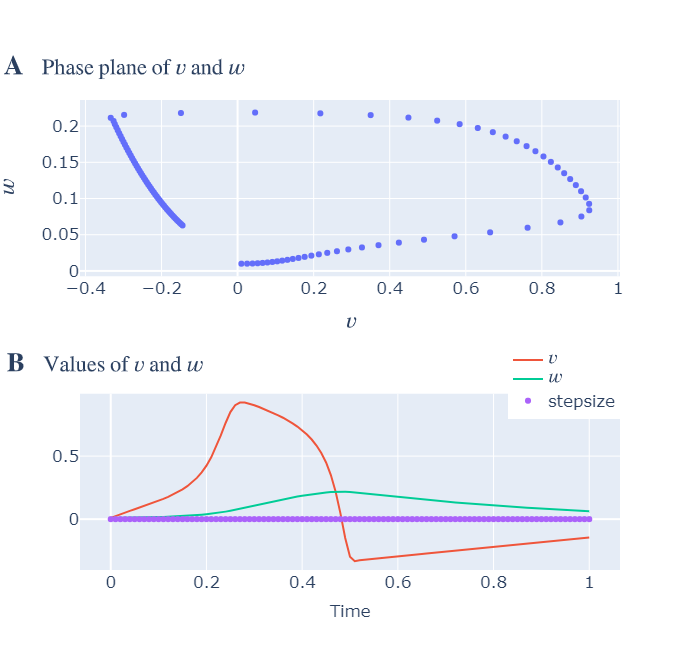
\includegraphics[width=0.95\columnwidth]{FHN_Euler_explicit}
    \caption{(\textit{A}) Phase plane of $v$ and $w$ by Euler's explicit method. (\textit{B}) Graph of $v$ and $w$ against time by Euler's explicit method.}
    \label{fig:FHN_Euler_explicit}
\end{figure}

From Figure \ref{fig:FHN_Euler_explicit} B, we can see that $v$, the excitation variable is excited in the early stage. While $v$ increases significantly, the change in $w$ is small. After $v$ reaches its peak and starts to reduce, $w$ increases slowly. This can be observed in both the phase plane (Figure \ref{fig:FHN_Euler_explicit} A) and the variable graph (Figure \ref{fig:FHN_Euler_explicit} B). When the variable $v$ starts to recover to its original value, $w$ is at its maximum. The scattering of points in the phase plane captures the feature of the model, where the change in $v$ is rapid while the change in $w$ is slow. When the change in $v$ is significantly larger than the change in $w$, the points are sparse. On the other hand, the points are packed when $w$ increases or decreases more than $v$. However, in the adaptive methods, such insights cannot be interpreted directly from the phase plane. Therefore, green triangles were plotted in Figure \ref{fig:FHN_adaptive} B to indicate the adapted mesh points. The mesh points are adapted towards large change in $v$ or $w$ over a short period of time.

\begin{figure}
    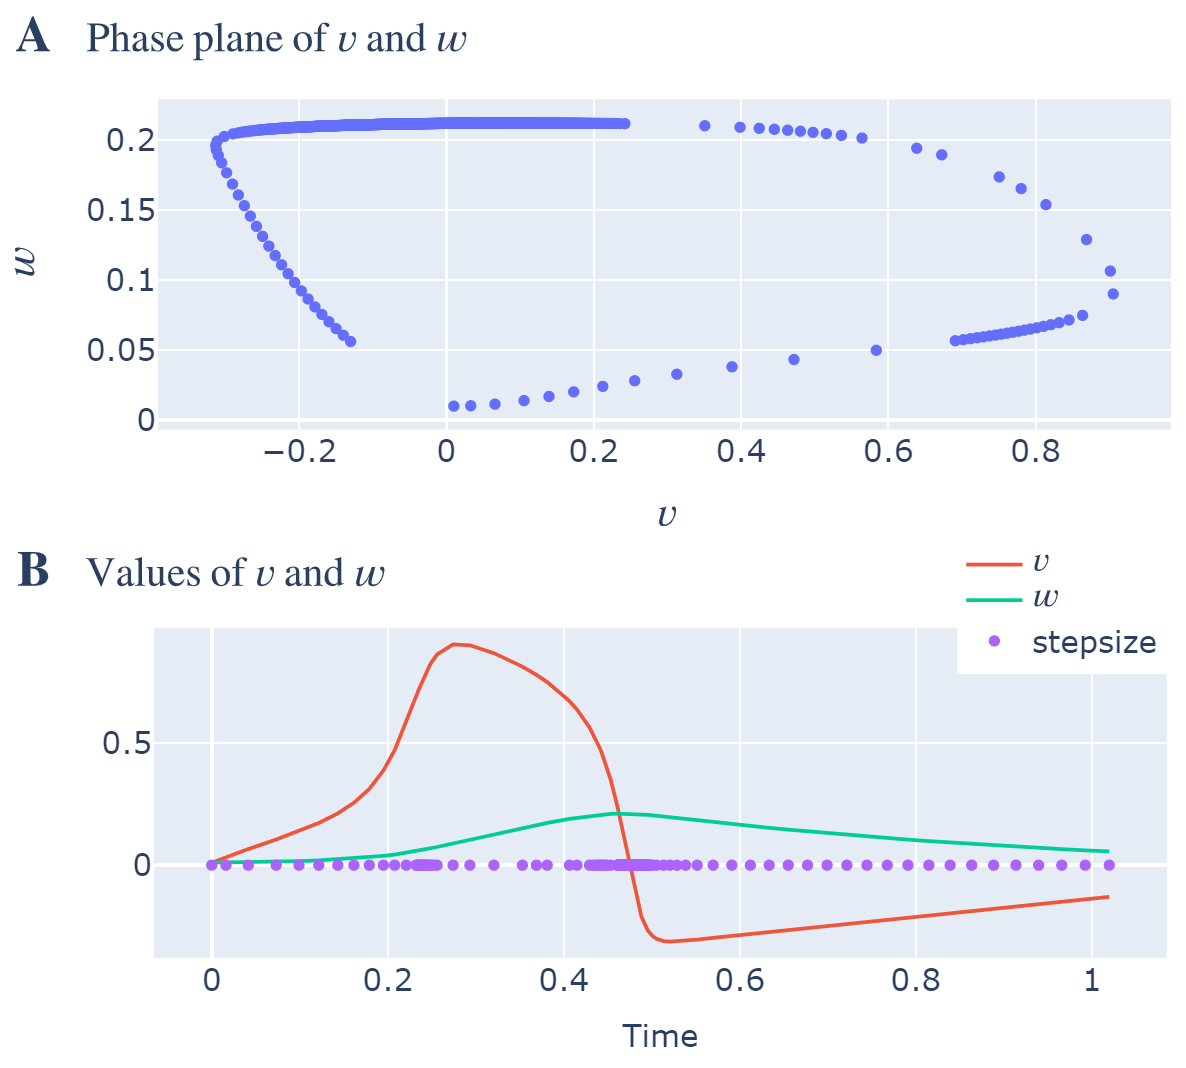
\includegraphics[width=0.95\columnwidth]{FHN_adaptive}
    \caption{(\textit{A}) Phase plane of $v$ and $w$ for adaptive method BS23. (\textit{B}) Graph of $v$ and $w$ against time for adaptive method BS23}
    \label{fig:FHN_adaptive}
\end{figure}

\section{Convergence of Fitzhugh-Nagumo model}
\label{sec:FHN-convergence}
A notebook (accessible from the link: \href{https://nbviewer.jupyter.org/github/FarmHJ/numerical-solver/blob/main/examples/fhn_model_convergence.ipynb}{\underline{\emph{Fitzhugh-Nagumo convergence notebook}}}) is created to test the convergence of the solution of the Fitzhugh-Nagumo model. Since the model has no analytical solution, it is tested against a reference solution. The reference solutions are assumed to be sufficiently accurate. For methods with fixed step size, which are the one-step methods and predictor-corrector method, the reference solutions are constructed by using a much smaller step size of $1^{-7}$, as compared to $1^{-5}$, the smallest step size for other numerical solutions. For methods with adaptive step size, reference solutions are obtained by using a much smaller tolerance value of $1^{-8}$, as compared to $1^{-5}$, the smallest tolerance value for other numerical solutions. This notebook shows the numerical solution computed for different methods at different step sizes or tolerance values. The numerical solutions are then compared with their respective reference solutions. In both methods, the error decreases as the step size or the tolerance value decreases, as shown in Figure \ref{fig:Euler_explicit_error} and Figure \ref{fig:adaptive_error}.

\begin{figure}
    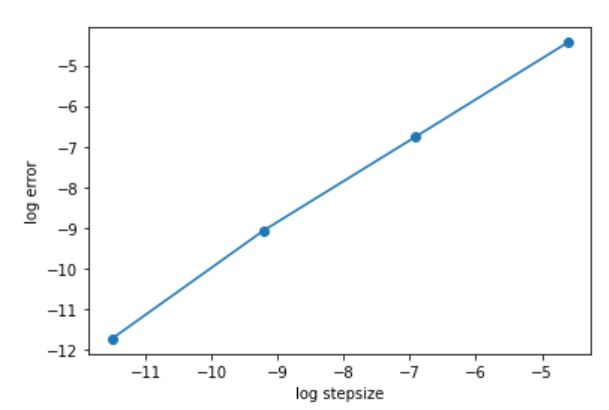
\includegraphics[width=0.95\columnwidth]{FHN_Euler_explicit_error_behaviour}
    \caption{Error at a mesh point for Euler's explicit method. The Fitzhugh-Nagumo model Eqs.~\eqref{eqn:FHN}-\eqref{eqn:FHN-end} is solved with Euler's explicit method at different step sizes. The error is the absolute difference between reference solution and numerical solution at $x=0.7$. The reference solution is taken at step size of $1^{-7}$. Note that $\log(1^{-7})\simeq-16.118$.}
    \label{fig:Euler_explicit_error}
 \end{figure}
\begin{figure}
   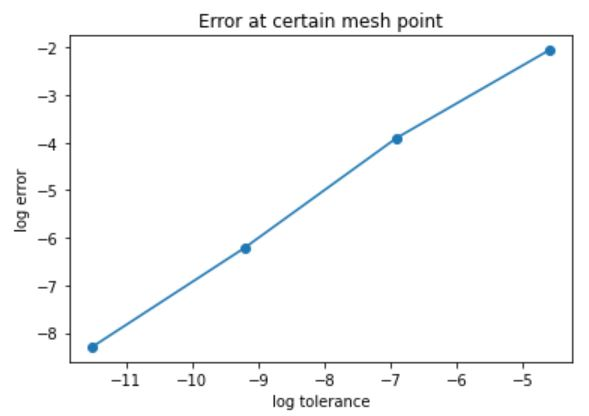
\includegraphics[width=0.95\columnwidth]{FHN_adaptive_error_behaviour}
   \caption{Sum of error for adaptive method BS23. The Fitzhugh-Nagumo model Eqs.~\eqref{eqn:FHN}-\eqref{eqn:FHN-end} is solved with BS23 method at different absolute tolerance values. The relative tolerance is fixed at $1^{-15}$. The error is the sum of absolute difference between reference solution and numerical solution at all mesh points. The reference solution is taken at relative tolerance of $1^{-8}$. Note that $\log(1^{-8})\simeq-18.421$.}
   \label{fig:adaptive_error}
\end{figure}